\documentclass{article}
\usepackage[utf8]{inputenc}
\usepackage[T1]{fontenc}
\usepackage{textcomp}
\usepackage[english, french]{babel}
\usepackage[babel=true]{csquotes}
\usepackage{tikz}
\usepackage{pgfplots}
\usepackage{array}
\usepgfplotslibrary{external} 
\tikzexternalize

\usepackage{color}
\usepackage{listings}

% Configuration de la coloration syntaxique du code
\definecolor{bleugris}{rgb}{.2,.4,.5}
\definecolor{colKeys}{rgb}{0,0,1}
\definecolor{colIdentifier}{rgb}{0,0,0}
\definecolor{colComments}{rgb}{0,0.5,1}
\definecolor{colString}{rgb}{0.6,0.1,0.1}

\newcommand{\nClass}[1]{{\color{bleugris}{\textsl{\textbf{#1}}}}}
\newcommand{\nParameter}[1]{{\color{gray}{\textbf{#1}}}}
\newcommand{\nMethod}[1]{{\color{gray}{\textbf{#1}}}}
\newcommand{\nConstant}[1]{\texttt{\uppercase{#1}}}
\newcommand{\nKeyword}[1]{\textsl{\textbf{#1}}}


\definecolor{lightgray}{rgb}{.9,.9,.9}
\definecolor{darkgray}{rgb}{.4,.4,.4}
\definecolor{purple}{rgb}{0.65, 0.12, 0.82}
\lstdefinelanguage{JavaScript}{
  keywords={break, case, catch, continue, debugger, default, delete, do, else, false, finally, for, function, if, in, instanceof, new, null, return, switch, this, throw, true, try, typeof, var, void, while, with},
  morecomment=[l]{//},
  morecomment=[s]{/*}{*/},
  morestring=[b]',
  morestring=[b]",
  ndkeywords={class, export, boolean, throw, implements, import, this},
  keywordstyle=\color{blue}\bfseries,
  ndkeywordstyle=\color{darkgray}\bfseries,
  identifierstyle=\color{black},
  commentstyle=\color{purple}\ttfamily,
  stringstyle=\color{red}\ttfamily,
  sensitive=true
}

\newcommand{\userlstset}[1]{
  \lstset{ %
    language=#1,                   % choose the language of the code
    identifierstyle=\color{colIdentifier},%
    basicstyle=\ttfamily\scriptsize, %
    keywordstyle=\color{colKeys},%
    stringstyle=\color{colString},%
    commentstyle=\color{colComments},%
    numberstyle=\tiny,              % the size of the fonts that are used for the line-numbers
    numbers=left,                   % where to put the line-numbers
    stepnumber=1,                   % the step between two line-numbers. If it is 1 each line will be numbered
    numbersep=5pt,                  % how far the line-numbers are from the code
    backgroundcolor=\color{white},  % choose the background color. You must add \usepackage{color}
    showspaces=false,               % show spaces adding particular underscores
    showstringspaces=false,         % underline spaces within strings
    showtabs=false,                 % show tabs within strings adding particular underscores
    %frame=single,                  % adds a frame around the code
    tabsize=2,                      % sets default tabsize to 2 spaces
    captionpos=b,                   % sets the caption-position to bottom
    breaklines=true,                % sets automatic line breaking
    breakautoindent = true,         %
    breakatwhitespace=false,        % sets if automatic breaks should only happen at whitespace
    escapeinside={\@}{\@},         % if you want to add a comment within your code
    % texcl=true
  } %
}

\newcommand{\ic}[1]{\lstinline|#1|}

\lstnewenvironment{code}[1][JavaScript]{%
  \userlstset{#1}%
}{%
}

\begin{document}

In this document, we want show the difference of response time of the different methods for calling a function using the event loop.

There is 4 ways to call a function, 3 queuing this function on the event loop, and directly calling the function.
From the documentation, here is a brief explanation of the differences, illustrated in Figure \ref{fig:eventloop}.

\begin{itemize}
  \item[direct call] straightforward.
  \item[\textit{nextTick}] The function \texttt{process.nextTick} pushes the function passed as an argument to the very beginning of the next loop.
    That means, the current execution will continue until it ends, then the queued function will be executed before anything else, including \textit{IO Operations}.
  \item[\textit{setImmediate}] The function \texttt{setImmediate} pushes the function passed as an argument to the next event loop, just after \textit{IO Operations} finished.
  \item[\textit{setTimeout}] The function \texttt{setTimeout} pushes the function passed as an argument to the next event loop to be executed after a certain delay, specified as an argument.
    This delay can't be respected, thus even when it's zero, the queued function will be executed after averything else.
\end{itemize}

\begin{figure}[h!]
  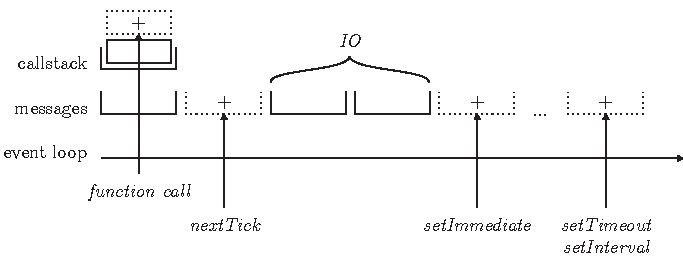
\includegraphics[width=\linewidth]{eventloop.pdf}
  \caption{Javascript event loop details}
  \label{fig:eventloop}
\end{figure}

We tested the order of execution of these different queueing method with the listing \ref{lst:order}.
Even if it's in complete contradiction\footnote{setImmediate(callback, [arg], [...]) : To schedule the "immediate" execution of callback after I/O events callbacks and before setTimeout ... However, this difference might come from a difference in the implementation, the last documentation version is 0.11.26, while my version of node is 0.10.22} with the node manual, the order appears to be the following :
Results from the execution of listing \ref{lst:order}.
\texttt{
0 directCall
1 nextTick
2 setTimeout
3 setImmediate
}

\begin{code}[Javascript, caption={test order of execution},label={lst:order}]
var index = 0;

function test(name) {
  console.log((index++) + " " + name);
}

setImmediate(function() {
  test("setImmediate");
})

setTimeout(function() {
  test("setTimeout");
}, 0);

process.nextTick(function() {
  test("nextTick");
})

test("directCall");
\end{code}


We tested the difference of run time between these different methods.
On Figure \ref{fig:eventloop} we can see the difference between the time spent inside a function, and the time spent between the call and the end of this function.

We base our test on the \texttt{wait} function in listing \ref{lst:wait}.
This function was called by different calling function in listings \ref{lst:direct}, \ref{lst:next}, \ref{lst:timeout} and \ref{lst:immediate}.
We probed the time just before the callings functions, and just after exiting the \texttt{wait} function.

\begin{code}[Javascript, caption={wait function},label={lst:wait}]
function wait(duration, start, _cb) {
  var iterations = 0;
  var end = time.now() + duration * 1000;
  while( time.now() < end ) {
    iterations++;
  }
  return _cb(start, time.now());
}
\end{code}


\begin{code}[Javascript, caption={Direct call},label={lst:direct}]
function(fn, args) {
  args[1] = time.now();
  fn.apply(null, args);
}
\end{code}

\begin{code}[Javascript, caption={\textit{nextTick}},label={lst:next}]
function(fn, args) {
  process.nextTick((function(fn, args) {
    args[1] = time.now();
    return function() {
      fn.apply(null, args);
    }
  })(fn, args));
},
\end{code}

\begin{code}[Javascript, caption={\textit{setTimeout}},label={lst:timeout}]
function(fn, args) {
  args.unshift(0)
  args.unshift(fn);
  args[3] = time.now();
  setTimeout.apply(null, args);
}
\end{code}

\begin{code}[Javascript, caption={\textit{setImmediate}},label={lst:immediate}]  
function(fn, args) {
  args.unshift(fn);
  args[2] = time.now();
  setImmediate.apply(null, args);
},
\end{code}

On the figure \ref{fig:plot}, we can see that while \textit{nextTick} and \textit{setImmediate} are one order of magnitude slower than a direct call, \textit{setTimeout} is about 3 order of magnitude slower than a direct call.  

\begin{figure}
  \begin{tikzpicture}
\begin{axis}[xlabel = value passed to \texttt{wait} function (ms), ylabel = Median of response time minus\\value passed in \texttt{wait} function (ms), legend style = {at={(0.5,-0.5)}, anchor=center}]
\addplot[mark = x, color = blue] coordinates {(10, 0.0030000000000001137) (9, 0.0039999999999995595) (8, 0.0030000000000001137) (7, 0.0039999999999995595) (6, 0.001000000000000334) (5, 0.001000000000000334) (4, 0.001000000000000334) (3, 0.0009999999999998899) (2, 0.0009999999999998899) (1, 0.0009999999999998899) (0, 0.001)};
\addplot[mark = x, color = red] coordinates {(10, 0.0259999999999998) (9, 0.018000000000000682) (8, 0.018000000000000682) (7, 0.017999999999999794) (6, 0.019000000000000128) (5, 0.017999999999999794) (4, 0.019000000000000128) (3, 0.017999999999999794) (2, 0.019000000000000128) (1, 0.018999999999999906) (0, 0.018)};
\addplot[mark = x, color = green] coordinates {(10, 1.2850000000000001) (9, 1.263) (8, 1.2889999999999997) (7, 1.2759999999999998) (6, 1.242) (5, 1.298) (4, 1.2489999999999997) (3, 1.274) (2, 1.251) (1, 1.255) (0, 1.255)};
\addplot[mark = x, color = yellow] coordinates {(10, 0.05599999999999916) (9, 0.06300000000000061) (8, 0.05599999999999916) (7, 0.05600000000000005) (6, 0.05999999999999961) (5, 0.05900000000000016) (4, 0.05400000000000027) (3, 0.05799999999999983) (2, 0.05799999999999983) (1, 0.05600000000000005) (0, 0.058)};
\legend{direct call, nextTick, setTimeout, setImmediate};
\end{axis}
\end{tikzpicture}

\label{fig:plot}
\end{figure}

On the \ref{fig:data}, we can see the resulting data of this experiment

\begin{figure}
\[\begin{array}{cccc}
direct call & nextTick & setTimeout & setImmediate \\
\hline \\
0.001 & 0.018 & 1.255 & 0.058 \\
0.0009999999999998899 & 0.018999999999999906 & 1.255 & 0.05600000000000005 \\
0.0009999999999998899 & 0.019000000000000128 & 1.251 & 0.05799999999999983 \\
0.0009999999999998899 & 0.017999999999999794 & 1.274 & 0.05799999999999983 \\
0.001000000000000334 & 0.019000000000000128 & 1.2489999999999997 & 0.05400000000000027 \\
0.001000000000000334 & 0.017999999999999794 & 1.298 & 0.05900000000000016 \\
0.001000000000000334 & 0.019000000000000128 & 1.242 & 0.05999999999999961 \\
0.0039999999999995595 & 0.017999999999999794 & 1.2759999999999998 & 0.05600000000000005 \\
0.0030000000000001137 & 0.018000000000000682 & 1.2889999999999997 & 0.05599999999999916 \\
0.0039999999999995595 & 0.018000000000000682 & 1.263 & 0.06300000000000061 \\
0.0030000000000001137 & 0.0259999999999998 & 1.2850000000000001 & 0.05599999999999916\\
\end{array}\]
\label{fig:data}
\caption{Raw data of the experiment}
\end{figure}
\end{document}
